\section{Medical Imaging Techniques}

\subsection{X-Ray imaging}
X-ray imaging is a medical imaging method that uses X-ray radiation to generate images. X-ray photons are generated using a X-ray tube which consist of an anode and a cathode on opposite sides, with vacuum in the space between them. Electrons are liberated when the cathode is heated up, and accelerate at a high speed toward the anode. When the electrons hit the anode (which usually consist of one of the metals tungsten, copper or molybdenum) about 1\% of the energy is converted into X-ray photons while the rest dissipates as heat. The X-ray photons are directed towards the patient, which is located between the X-ray tube and a detector (digital film). The X-ray travels through the body, some of it being absorbed and the rest hits the detector. The parts of the body with high density absorbs most of the X-ray directed towards it, while soft tissues such as muscle and fat absorbs some of it depending on the type of tissue and its density. The detector acts as a digital film which represents the final image as white where the X-ray energy was absorbed by the body, and dark in places with little absorbation (e.g. liquid and air). The X-ray image can thus be seen as the "shadow" of the released X-ray energy. 

Even if the soft tissues does not absorb as much of the X-ray as the hard tissues, they still absorb some, so if a low energy photon source were used, it would be difficult to see the difference of hard and soft tissues in the resulting X-ray image. This is why X-ray on bones and other hard tissues requires a photon source of high energy, but high energy means more radiation. A side-effect of X-ray imaging is the ionizing radiation from the X-rays, but conventional X-ray imaging does not require a large amount of radiation. Another disadvantage is that conventional X-ray imaging can only be used to create 2D images, which limits the amount of information gained. Advantages with X-ray imaging is that it is very fast to use and good at bone imaginng. Thus, X-ray imaging is widely used to detect bone fractures and by dentists to exam teeth.

\subsection{Computed Tomography}
A computed tomography (CT) machine consist of a X-ray source (emitter) that generates X-ray and releases it towards the patient. The detector array at the opposite side receives the X-ray not absorbed by the patient. The machine rotates around the patient while releasing X-ray photons to get information from all directions. The detector array (scintillator) transforms the X-rays into proportionally strong electric current which is represented as image slices. By moving the table step by step a full 3D volume can be created by combining the 2D slices together. 

The advantages by using CT over a normal X-ray scan is that CT can take images in any direction, and that the result is a volume of data. Another advantage is the high contrast of the resulting images, CT can differentiate between tissues with less than 1\% density difference. But better quality comes with a cost, increasing the quality of the images requires an increase in the amount of radiation. So there is always a tradeoff between noise in the images and the dosage of radiation. As mentioned before, X-rays are ionizing, and the high amount of ionizing radiation from CT is its biggest disadvantage. MRI is sometimes preferred over CT for small children, since the ionizing radiation effects younger people more.
\begin{figure}[h!]
\centering
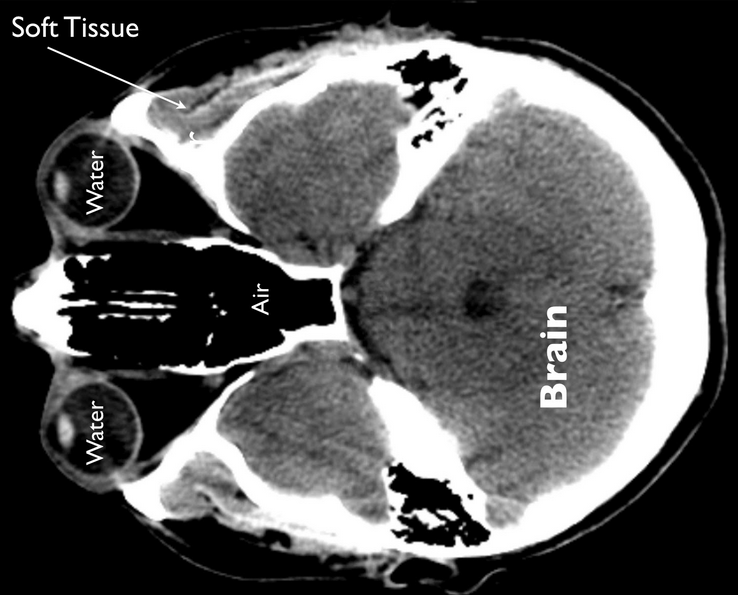
\includegraphics[width=0.45\textwidth]{backgroundTheory/medicalImaging/CTimageRot}
\caption{CT image of a head.}
\label{CTimage}
\end{figure}
Unlike conventional X-ray imaging which is mostly used to represent teeth and bone, CT is used more broadly. CT is for example used to image the heart, abdomen, acute and chronic changes in lung, detecting tumors in different parts of body, in addition to bone fractures. Figure \ref{CTimage} depicts a regular CT image of the head.

\subsection{Magnetic Resonance Imaging}
All electrons, protons and neutrons have an angular momentum around their own axis, i.e. they have a spin. All charged objects with a spin and an odd number mass number creates a magnetic field around themselves. These small magnetic fields are exploited by a MRI machine to generate the MRI signal. These tiny magnetic fields are randomly aligned when no external force is acting on them.

If a small magnetic field is inside a much stronger homogenous magnetic field it will align itself according to the strong one. This is the idea behind MRI. The fact that hydrogen is the most abundant element in the body when considered as number of atoms, and its nucleus only consist of a single proton makes hydrogen the most sensitive atom to MRI machines. 

The magnetic fields generated by MRI machines used clinically today vary from 0.2 to 3 tesla, and using stronger magnetic fields results in lower signal-to-noise ratio. The homogenous magnetic field, \(B_0\), generated by the MRI machine is aligned in a certain direction referred to as the longitudinal direction. When \(B_0\) is turned on, the hydrogen protons in the patient's body are aligned parallel with it, i.e. in the longitudinal direction. Most of the protons will align their magnetic field in the longitudinal direction, causing a net magnetisation \(M_z\) aligned parallel with \(B_0\) (\(M_z = M_0\)), while some will align in the opposite (antiparallel) direction. The favorable state of the protons is when they are parallel with \(B_0\), which is the less energetic and more stable state. While \(B_0\) is turned on, a small radio frequency pulse (RF-pulse) is applied through a coil perpendicular to \(B_0\), towards the area of the body to be examined. This RF-pulse has the same frequency as the spin, or nuclear precession, of the hydrogen protons, thus affecting only the hydrogen nucleus. The hydrogen protons aligned with \(B_0\) will absorb this RF-pulse and jump to a higher energy state, and as a result align in a direction away from \(B_0\), causing the net magnetisation \(M_z\) to rotate away from the longitudinal direction. The amount of rotation depends on the strength and length of the RF-pulse. The RF-pulse can therefore be used to adjust the direction of net magnetisation to any angle. When the RF-pulse is turned off, the absorbed energy is released, resulting in the protons to return (relax) to being re-aligned with \(B_0\). The RF-pulse is continously turned on and off, and the energy emitted (MR-signal) when relaxing is picked up by receiver coils, processed by a computer and stored as a 3D data volume. 

In addition to the homogenous \(B_0\) field there are additional smaller magnetic fields called gradient fields. The purpose of these non-homogenous gradient fields is to determine the exact position of where to get a 2D slice from. A gradient field changes the precession of the hydrogen protons along the axis it is applied, and by sending out RF-pulses targeting these hydrogen protons the exact position of the patients body to get a 2D slice from is determined. Moreover, the gradient fields and the RF-pulse can also be used to determine the thickness of the 2D slices. 

The advantage of MRI over CT is that there is no ionizing radiation associated with it. A disadvantage is that people with metal implants can not use MRI because of the strong magnetic field. Another disadvantage is that the imaging process takes long time, which is problematic for people with claustrophobia since the patient have to be inside the machine.

\subsection{T1 and T2 weighted images}
The time interval between two successive RF-pulses is called the repetition time (\(T_R\)), and the time taken from the RF-pulse is applied to the peak of the signal received by the coil is the echo time (\(T_E\)). The time taken after a RF-pulse for the net magnetisation \(M_z\) to re-align with \(B_0\) is called the longitudinal or spin-lattice relaxation time. The magnetisation in the longitudinal plane (z-axis) is given by
\begin{equation}
M_z = M_0(1-e^{-t/T_1}),
\end{equation}
where \(T_1\) is the time taken for \(M_z\) to recover \(1-e^{-1} = 63\%\) of the equilibrium net magnetisation \(M_0\). \(T_1\) varies for protons of different tisse types. This is measured and used as the main source of tissue contrast information in \(T_1\)-\textit{weighted} images. \(T_1\)-weighted images are created at the time of the greatest difference between the \(T_1\) values of the tissues being examined, by using short \(T_R\) and \(T_E\). Increasing the magnetic field \(B_0\) increases \(T_1\), hence increasing the strength of \(B_0\) gives better contrast in \(T_1\)-weighted images.

Neighbouring molecules causes the hydrogen protons attached to different types of molecules to experience slightly different local magnetic fields. As a result, these hydrogen protons will precess at slightly different frequencies. This causes the spins to dephase and decrease the net transverse (xy-plane) magnetisation right after the RF-pulse is turned off, and is called transverse or spin-spin relaxation. This decay of magnetisation in the transverse plane is defined as
\begin{equation}
M_{xy} = M_0 \, e^{-t/T_2},
\end{equation}
where \(T_2\) is the time taken for transverse magnetisation to reach \(e^{-1} = 37\%\) of its initial value. The contrast in \(T_2\)-weighted images are determined by differences in \(T_2\) relaxation times of different tissue types, and is taken when the difference in the \(T_2\) values is greatest.

The difference of \(T_1\) and \(T_2\)-weighted images is illustrated in figure \ref{tweight} (from \cite{eng08}). Both images were taken with magnetic fields of 1.5 tesla. 
\begin{figure}[h!]
\centering
\begin{minipage}{.4\textwidth}
\begin{tabular}{c}
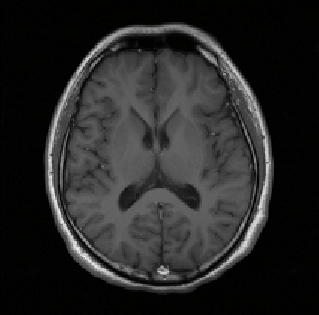
\includegraphics[width=\textwidth]{backgroundTheory/medicalImaging/T1} \\
(a)
\end{tabular}
\end{minipage}
\begin{minipage}{.4\textwidth}
\begin{tabular}{c}
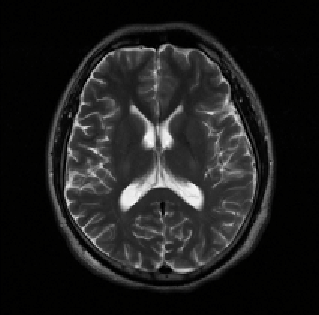
\includegraphics[width=\textwidth]{backgroundTheory/medicalImaging/T2} \\
(b)
\end{tabular}
\end{minipage}
\caption{(a): T1-weighted image, (b): T2-weighted image}
\label{tweight}
\end{figure}
In \(T_1\)-weighted images, fluids (such as the cerebrospinal fluid in figure \ref{tweight} a) are dark and fat-based tissues are brighter. This gives clear boundaries between different tissue types, and is thus used to represent anatomical structures. Fluids are very bright and tissues are mid gray in \(T_2\)-weighted images. Therefore, \(T_2\)-weighted are used to demonstrate pathology.